% ****** Start of file apssamp.tex ******
%
%   This file is part of the APS files in the REVTeX 4.1 distribution.
%   Version 4.1r of REVTeX, August 2010
%
%   Copyright (c) 2009, 2010 The American Physical Society.
%
%   See the REVTeX 4 README file for restrictions and more information.
%
% TeX'ing this file requires that you have AMS-LaTeX 2.0 installed
% as well as the rest of the prerequisites for REVTeX 4.1
%
% See the REVTeX 4 README file
% It also requires running BibTeX. The commands are as follows:
%
%  1)  latex apssamp.tex
%  2)  bibtex apssamp
%  3)  latex apssamp.tex
%  4)  latex apssamp.tex
%
\documentclass[%
 reprint,
%superscriptaddress,
%groupedaddress,
%unsortedaddress,
%runinaddress,
%frontmatterverbose, 
%preprint,
%showpacs,preprintnumbers,
%nofootinbib,
%nobibnotes,
%bibnotes,
 amsmath,amssymb,
 aps,
%pra,
%prb,
%rmp,
%prstab,
%prstper,
%floatfix,
]{revtex4-1}

\usepackage{graphicx}% Include figure files
\usepackage{dcolumn}% Align table columns on decimal point
\usepackage[spanish]{babel}
\selectlanguage{spanish} 
\usepackage[utf8]{inputenc}
\usepackage{bm}% bold math
%\usepackage{hyperref}% add hypertext capabilities
%\usepackage[mathlines]{lineno}% Enable numbering of text and display math
%\linenumbers\relax % Commence numbering lines
\usepackage{float}
%\usepackage[showframe,%Uncomment any one of the following lines to test 
%%scale=0.7, marginratio={1:1, 2:3}, ignoreall,% default settings
%%text={7in,10in},centering,
%%margin=1.5in,
%%total={6.5in,8.75in}, top=1.2in, left=0.9in, includefoot,
%%height=10in,a5paper,hmargin={3cm,0.8in},
%]{geometry}
\usepackage[font=footnotesize,labelfont=bf]{caption}
\usepackage{hyperref}
\newcommand{\subtitle}[1]{%
\posttitle{%
    \par\end{center}
\begin{center}\large#1\end{center}
\vskip0.5em}%
}
\begin{document}

%\preprint{APS/123-QED}

\title{Doble Rendija\\ \textit{Estudio de la dualidad de onda partícula} }% Force line breaks with \\

%\subtitle{Estudio de la dualidad de onda partícula}

\author{Jose Alejandro Montaña Cortés}
\email{ja.montana@uniandes.edu.co}
% \altaffiliation[Also at ]{Departamento de Física, Universidad de los Andes}
\author{Jesús David Rincón Puche}%
\email{jd.rincon883@uniandes.edu.co}
\affiliation{Departamento de Física, Universidad de los Andes}%

%\collaboration{}%\noaffiliation

\date{\today}% It is always \today, today,
             %  but any date may be explicitly specified

\begin{abstract}



\end{abstract}
\maketitle
%\tableofcontents

%---------------------INTRODUCCIÓN------------------
\section{Introducción}
Desde mediados de 1600 hasta inicios de 1900 se discutió si la luz debía ser considerada como una onda o como una partícula. Tal discusión se originó cuando el científico holandés C.Huygens conoce a  I. Newton en 1689, en esta fecha, Huygens publica su  teoría ondulatoria de la luz. Por otra parte, Newton opta por describir la naturaleza de la luz por medio de lo que él llamó “corpúsculos”. No obstante, con los desarrollos posteriores de Fresnel y Maxwell se ratificaba el comportamiento de tipo ondulatorio en la luz, con lo cual a finales de 1800 se creía que esta “dualidad” en la teoría parecía haberse esclarecido. Sin embargo, con el descubrimiento del efecto Compton y el efecto fotoeléctrico la descripción de la luz como cuantos de luz o como “corpúsculos” volvió a tomar fuerza. Posteriormente gracias al desarrollo de la mecánica cuántica el concepto de tomar a una partícula como un objeto que además exhibe propiedades de onda fue bien acogida por la comunidad científica y esta tomó bastante fuerza a mediados de 1900. En este experimento se estudiará las propiedades de onda y partícula que posee la luz al efectuar un montaje similar al propuesto por Young en 1803 en donde se hace pasar un haz de luz por medio de una doble rendija y así hacer uso de la teoría de difracción e interferencia de la óptica clásica para explicar el fenómeno. Posterior a esto con el fin de observar el comportamiento de partícula se envía una cantidad “pequeña” de fotones para que pase por una de las rendijas en un momento dado, esto con el fin de mostrar la dualidad de onda partícula de la luz.
\section{Desarrollo teórico}
\begin{figure}[h]
\center{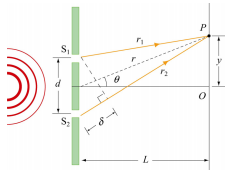
\includegraphics[width=0.4\textwidth]
{../Figuras/double_rendija.PNG}}
\caption{\label{doble rendija} Diagrama geométrico de la luz pasando por la doble rendija, de acá se puede deducir que $\delta=r_2-r_1\approx d\sin(\theta)$, lo cual es valido si la razón entre distancia entre las rendijas y la distnacia al detector es pequeña ($d/L\ll 1$)   (tomado de \cite{MIT}).}
\end{figure}
Gracias al desarrollo de la electrodinámica, se logró entender el comportamiento de la luz por medio de una ondas electromagnéticas. Debido a esto, la intensidad de la luz proveniente de 2 fuentes distintas\footnote{Para nuestro caso 2 rendijas}, puede escribirse como:
\[I(z,t)=\vec{E}(z,t)\cdot \vec{E}(z,t),\]
pero dado que $I(z,t)$ varia muy rápido en el tiempo, se toma el promedio de esta cantidad sobre un tiempo $T'$ grande, múltiplo del periodo $T$, con lo cual se tiene entonces que:
\[I(z)\propto\ \frac{1}{T'}\int_{0}^{T'}\vec{E}(z,t)\cdot \vec{E}(z,t) dt \sim \langle \vec{E}\cdot \vec{E}\rangle.\]
Dado que acá $\vec{E}$ representa el campo total y este a su vez está conformado por la suma de dos campos (uno de cada fuente), se tiene entonces que la intensidad está dada por,
\begin{equation*}
  \langle \vec{E}\cdot \vec{E}\rangle = \langle (\vec{E_1}+\vec{E_2})\cdot (\vec{E_1}+\vec{E_2})\rangle,
\end{equation*}
\begin{equation}
I\sim \langle E_1^2\rangle+\langle E_2^2\rangle+2\langle \vec{E_1}\cdot  \vec{E_2}\rangle,
\label{difrac}
\end{equation}
donde el térmico cruzado $\langle \vec{E_1}\cdot  \vec{E_2}\rangle$ es el que origina la interferencia. Con el fin de determinar una función para $I$ que contenga valores fácilmente medibles en el laboratorio, es posible escribir $\vec{E_1}$ y $\vec{E_2}$ en términos de ondas monocromáticas y coherentes.
\begin{align}
\vec{E_1}&=\vec{E_0}\sin(\omega t)   &  \vec{E_2}&=\vec{E_0}\sin(\omega t+ \phi),
\label{campos electricos}
\end{align}
con lo que efectuando la integral y reescribiendo el producto de los  se tiene entonces que \footnote{En donde se efectuó la integral
\[ \frac{1}{T}\int_{0}^{T}\sin^2\left(\omega t+\frac{\phi}{2}\right)=\frac{1}{2}\]
}
\begin{multline}
I\sim  \langle \vec{E}\cdot \vec{E}\rangle = 4E_0^2 \cos^2\left(\frac{\phi}{2}\right)\langle\sin^2\left(\omega t+\frac{\phi}{2}\right)\rangle \\
=2E_0^2\cos^2\left(\frac{\phi}{2}\right).
\label{intensidad_1}
\end{multline}
Con esto se tiene entonces que para que haya interferencia de tipo constructiva, es necesario que $\phi=2\pi$, lo cual corresponde a una diferencia de camino de $\delta=\lambda$, donde $\lambda$ corresponde la longitud de onda de la luz y $\delta$ es la diferencia de caminos entre los dos campos eléctricos. Así de esta forma se deduce que
\begin{equation}
\phi = \frac{2\pi d}{\lambda}\sin\theta,
\label{relacion_fase}
\end{equation}
sustituyendo \eqref{relacion_fase} en \eqref{intensidad_1} se tiene que
\begin{equation}
I=I_0\cos^2\left(\frac{\pi d \sin\theta}{\lambda}\right).
\label{interferencia}
\end{equation}
De una forma similar, se puede mostrar que para una sola rendija la intensidad  de la luz está dada por
\begin{equation}
I=I_0\left(\frac{\sin\alpha}{\alpha}\right)^2,
\label{difraccion}
\end{equation}
en donde
\begin{equation}
\alpha=\frac{\pi a}{\lambda}\sin\theta,
\end{equation}
\begin{figure}[h]
\center{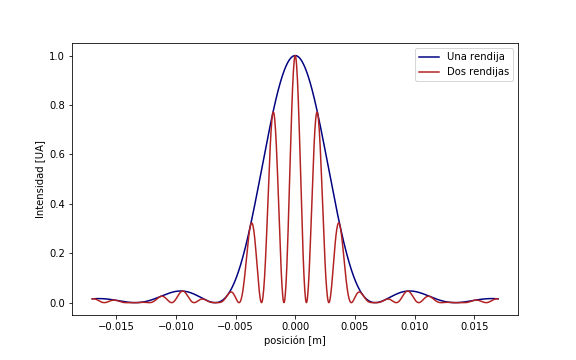
\includegraphics[width=0.4\textwidth,trim={1.5cm 0 1.5cm 0}]
{../Figuras/Ejemplo_interferencia.png}}
\caption{\label{ejemplo interferencia} Ejemplo de la intensidad predicha por la ecuación \eqref{Intensidad_total} para el caso de las 2 rendijas (roja) y \eqref{difraccion} para el caso de una rendija (azul).}
\end{figure}
con $a$ la longitud de la rendija por la que pasa la luz. Por ultimo se tiene que la intensidad del patrón de luz debido a la difracción y la interferencia es el producto de las ecuaciones \eqref{interferencia} y \eqref{difraccion}
\begin{equation}
I=I_0\left(\frac{\sin\alpha}{\alpha}\right)^2\cos^2\left(\frac{\pi d \sin\theta}{\lambda}\right).
\label{Intensidad_total}
\end{equation}
Las ecuaciones \eqref{Intensidad_total} y \eqref{difraccion} se muestran en la figura \ref{ejemplo interferencia}, ambas gráficas son hechas con parámetros idénticos para así observar la diferencia en los patrones de interferencia de una rendija y dos rendijas. Con estos resultados se tiene entonces que el patrón esperado a observar ha de ser similar\footnote{No se espera que siga este patrón a la perfección dado que la fuente que se usa no es necesariamente coherente (tanto espacial como temporal)} al de la figura \ref{ejemplo interferencia} para el caso de 2 rendijas. 
% trim={<left> <lower> <right> <upper>}

%-----------------RESULTADOS----------------------
\section{Resultados y Análisis}
asfsdsdffs
\begin{figure}[ht]
\center{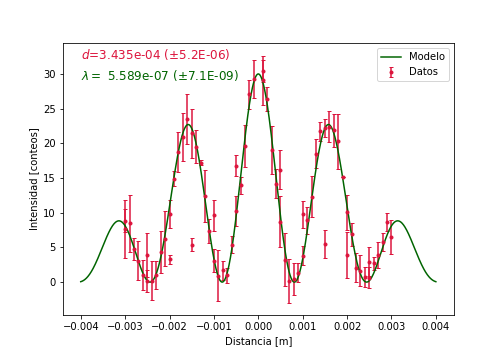
\includegraphics[width=0.4\textwidth]
{../Figuras/Interferencia_verde.png}}
\caption{\label{distribucion} .}
\end{figure}
\begin{figure}[ht]
\center{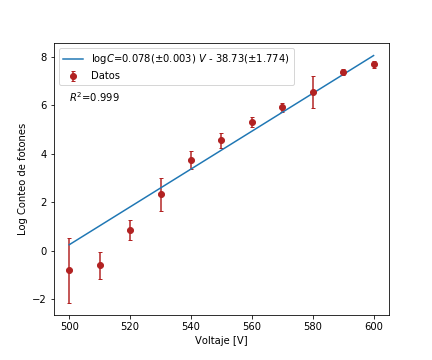
\includegraphics[width=0.4\textwidth]
{../Figuras/fotomultiplicador.png}}
\caption{\label{distribucion} .}
\end{figure}
\begin{figure}[ht]
\center{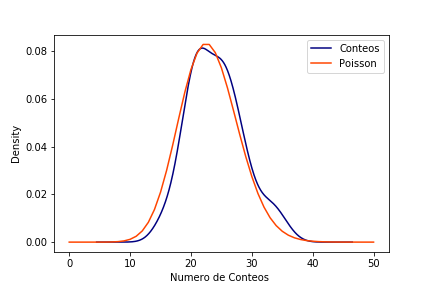
\includegraphics[width=0.4\textwidth]
{../Figuras/Distribucion.png}}
\caption{\label{distribucion} .}
\end{figure}
\begin{figure}[ht]
\center{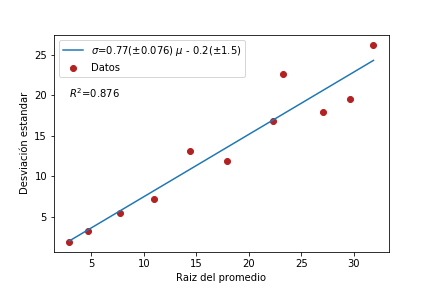
\includegraphics[width=0.4\textwidth]
{../Figuras/sqrt_promedio_std.png}}
\caption{\label{distribucion} .}
\end{figure}
%---------------CONCLUSIONES-------------------

\section{Conclusiones}
asdasdasd
%Se deben contestar las preguntas planteadas inicialmente o dar las razones por las cuales no es posible hacerlo. Las conclusiones deben ser necesariamente una consecuencia del experimento realizado, es decir que no se deben tocar aspectos que no se hayan expuesto en la sección de resultados y análisis. Si escribe algo que no se encuentra en la sección de resultados y análisis, esto quiere decir que hace falta incluir material en resultados y análisis. Concluir únicamente aspectos pertinentes a su trabajo en el laboratorio; evite generalizaciones que no hablan concretamente de lo que usted hizo o midió.

\begin{thebibliography}{9}
\bibitem{opticaondulatoria}
Université Moulay Ismaïl, 2017
\url{https://www.overleaf.com/project/5c58b017b206d66446cbc4bd}
\bibitem{MIT} 
Massachusetts Institute of Technology
\url{http://web.mit.edu/viz/EM/visualizations/coursenotes/modules/guide14.pdf}
\end{thebibliography}


\end{document}
%
% ****** End of file apssamp.tex ******
